\section{Positioning the Receiver Indexer}

Receiver Indexer (RI) carousel has four defined positions for each of the receivers it hosts. By selecting the frequency band on CAM’s  GUI during building of a subarray you are selecting a receiver position mounted on the indexer. Currently we are using L-band and UHF-band for observations and S-band is still being integrated. The raw angles for receivers when they are indexed are:
\begin{itemize}
\item{} L band = 40deg
\item{} X band = 80deg
\item{} U band = 120deg
\item{} S band = 0deg
\end{itemize}

There is no X$-$band receiver installed and X$-$band position is used for parking antennas for the flight arrival and departure on site. 

In order to index the receiver to be used for the observation, On the \server{obs} machine \server{obs.mkat.karoo.kat.ac.za},  run
\begin{lstlisting}[style=DOS]
ipython
Import katuilib
configure_cam('camcam', 'all')
cam.m0xx.req.mode('STOP') 
cam.m0xx.req.select_band('l', timeout=60)   
cam.m0xx.req.ap_set_indexer_position('l', timeout=60)

\end{lstlisting}
	

If you want to use the UHF band for the next observation, replace "l" with "u".  \\

The above-mentioned procedure can be used in instances where the receiver indexer becomes undefined, the \sensor{ap.indexer-position} sensor status on the GUI will be error. This can occur when the array is active, oftentimes during a running observation. 
\section{Switching LNAs on and off}

The Low Noise Amplifiers (LNAs) do not switch on automatically. They remain off until switched on by the operator. They are switched off automatically when the receiver warms up above 100\unit{K}. The 2nd stage amplifiers however, are switched on whenever the cooler is running. The most important sensor to worry about and report  when in error is \sensor{rsc.rxl.rfe1.temperature}  
and it must be below 30\unit{K} (ideally around 19\unit{K}). First, you need to create a configured ipython session by running on \component{obs} machine:
\begin{lstlisting}[style=DOS]
ipython
import katuilib
configure\_cam('camcam', 'all')

\end{lstlisting}


To turn on the LNAs, run:
\begin{lstlisting}[style=DOS]
cam.m0xx.req.rsc_rx(l or u)_lna_h_power('enable') 
cam.m0xx.req.rsc_rx(l or u)_lna_v_power('enable') 


\end{lstlisting}


In case you need to power cycle (turn off and then on again) the LNAs, run the following to turn the LNAs off:
\begin{lstlisting}[style=DOS]
cam.m0xx.req.rsc_rx(l or u)_lna_h_power('disable') 
cam.m0xx.req.rsc_rx(l or u)_lna_v_power('disable') 
\end{lstlisting}




To check in the CAM GUI if the LNA are switched on, select\\
 \textbf{Main menu} $>$ \textbf{ Sensor List}  $>$ \textbf{m0XX} $>$ \textbf{rsc.rx(l or u).lna$-$h.power$-$enabled nominal true}


The image in \textbf{Figure}~\ref{fig:image41} shows that LNA for \component{m006}, L, UHF and S-band receivers are switched on, i.e. enabled. 

\begin{figure}[!thb]
	\centering

	%\includegraphicsdpi{100}{}{bur1.png}     
	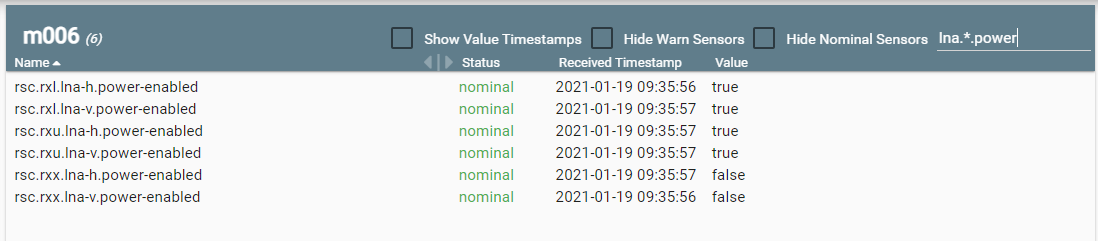
\includegraphics[scale=0.4]{Chapters/images/image41.png}
	
	%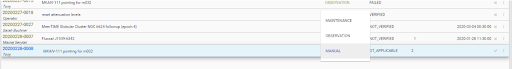
\includegraphics[resolution=100]{bur1.png}
	\caption{Sensor list showing LNA status}
	\label{fig:image41}
\end{figure} 
\section{ 2nd Stage Amplifiers}

To switch them on if they are off, again in the ipython session do the following:

\begin{lstlisting}[style=DOS]
cam.m0xx.req.rsc_rx(l)_amp2_h_power('enable')
cam.m0xx.req.rsc_rx(l)_amp2_v_power('enable')
\end{lstlisting}

To check if they are on, select\\
\sensor{Main menu} $>$ \sensor{Sensor List}  $>$ \sensor{m0XX} $>$ \sensor{rsc.rxl.amp2$-$h.power$-$enabled nominal true}

The image in \textbf{Figure}~\ref{fig:image51} shows that and stage amplifiers for \component{m006}, L, UHF and S-band receivers are switched on, i.e. enabled.

\begin{figure}[!thb]
	\centering
	
	%\includegraphicsdpi{100}{}{bur1.png}     
	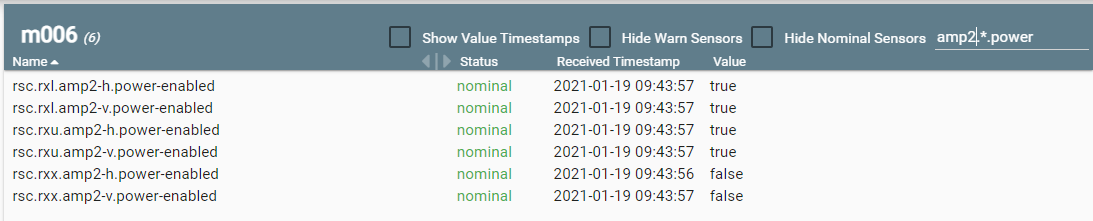
\includegraphics[scale=0.4]{Chapters/images/image51.png}
	
	%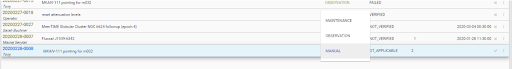
\includegraphics[resolution=100]{bur1.png}
	\caption{Sensor list showing stage 2 amplifiers}
	\label{fig:image51}
\end{figure} 

\section{ Helium Compressor}
The helium compressor supplies high pressure helium to the cryocoolers of the respective receivers. This means one helium compressor is connected to all working receivers on an AP. 

Hence if a fault occurs on the helium compressor, it will shut down causing all receivers (L-band, UHF-band and S-band) on the AP to warm up, making AP unusable for observations. There are usually two types of Helium compressor faults that occur:
\subsection{ Helium compressor pressure fault}
\textbf{Figure}~\ref{fig:He1} shows the sensors that go into error when a pressure fault occurs.

\begin{figure}[!thb]
	\centering
	%\includegraphicsdpi{100}{}{bur1.png}     
	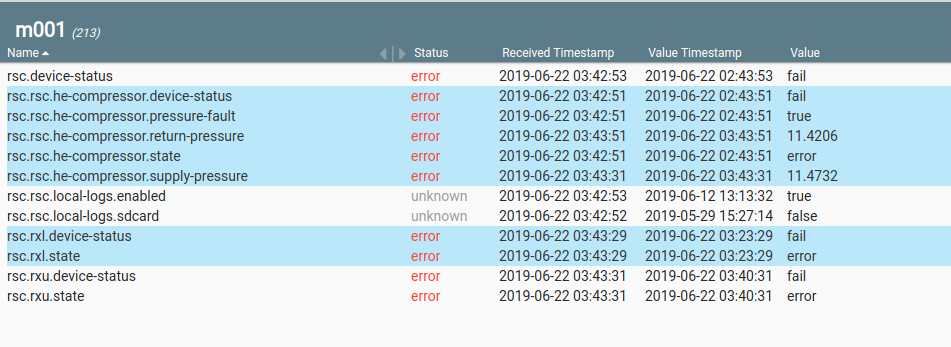
\includegraphics[scale=0.45]{Chapters/images/He1.png}
	
	%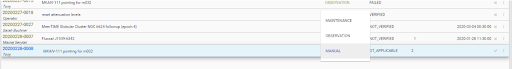
\includegraphics[resolution=100]{bur1.png}
	\caption{Receiver System Hellium presure errors}
	\label{fig:He1}
\end{figure}
\subsection{Helium compressor temperature fault}
\textbf{Figure}~\ref{fig:He2} shows the sensors that go into error when a temperature fault occurs.
Note the only difference in sensors between the two faults mentioned above is the sensor indicating the type of fault:
rsc.rsc.he-compressor-pressure-fault (for pressure faults)
rsc.rsc.he-compressor-temp-fault (for temperature faults)

If one of these faults thus occur, report the issue as such (you don’t have to also report that the receivers are warm in a separate report, since helium compressor faults automatically cause receivers to warm up).

\clearpage
\begin{figure}[!thb]
	\centering
	%\includegraphicsdpi{100}{}{bur1.png}     
	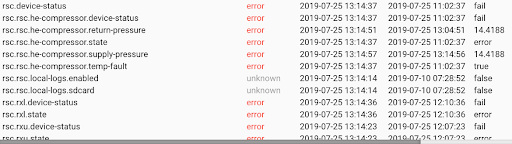
\includegraphics[scale=0.8]{Chapters/images/He2.png}
	
	%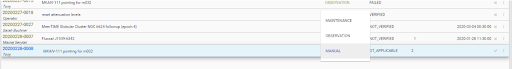
\includegraphics[resolution=100]{bur1.png}
	\caption{Receiver System temperature errors}
	\label{fig:He2}
\end{figure}



The following helium compressor sensors can be ignored (no action needed) when they go into error as they have no control value over the receivers and thus won’t affect observations in any manner:
\begin{itemize}
	\item{} \sensor{rsc.rsc.he-compressor.temperature1}
	\item{} \sensor{rsc.rsc.he-compressor.temperature2}
\end{itemize}

\section{ Receivers system debugging tools}
We have debugging tools for the receivers systems which technicians use to predict failures and reporting of the receiver system status.  (You can either choose the\file{rx\_daily} folder to view the daily receiver reports or the\file{rx\_monthly} folder to view the monthly receiver reports). The tool is written in an\package{IPYTHON} notebook and it is executed daily to provide daily reports. 

The following sensors can be ignored (no action needed as they are disabled and thus will show “unknown” status) as they have no control value over the receivers and thus won’t affect observations in any manner:
\begin{itemize}
	\item{} \sensor{rsc.rsc.local-logs.enabled}
	\item{} \sensor{rsc.rsc.local-logs.sdcard}
\end{itemize}

\begin{table}[h]
	
\caption{Receiver health by color coding.}
\label{tab:table1}

	\begin{tabular}[b]{|p{0.1cm}|p{0.6cm}|p{0.9cm}|p{0.2cm}|p{1.1cm}|p{1cm}|p{0.7cm}|p{0.2cm}|p{0.2cm}|p{1.1cm}|p{1.1cm}|p{1.1cm}|p{1.1cm}|}
		\hline
		
	\multicolumn{7}{|c|} {\done Green: Ok}& & & & &\\
		\hline
		\multicolumn{7}{|c|} {\hcya Yellow : System usable but report maintenance for schedule correction}& & & & &\\
		\hline	
		\multicolumn{7}{|c|} {\hcy Orange : System usable but monitor and report to maintanace if stte persist}& & & & &\\
		\hline
		\multicolumn{7}{|c|} {\hcyan Red : Do not use and report to maitenance immidiately}& & & & &\\
		\hline	
		\multicolumn{7}{|c|} {\hc Blue: Operator can change state}& & & & &\\
		\hline			
			& & & & & & & & & & &\\
		\hline
			 &m007 &Receiver System & 32& rsc& 14&rsc.current & 1& &  & &\\
		\hline
			& 1& Window&1 & & & rsc.voltage &1& & & &\\
		\hline
			& & & & & & & & & & &\\
		\hline
			& & & & & & & & & & &\\
		\hline
			& & & & & & & & & & &\\
		\hline
			& & & & & & & & & & &\\
		\hline
			& & & & & & & & & & &\\
		\hline
			& & & & & & & & & & &\\
		\hline
			& & & & & & & & & & &\\
		\hline
			& & & & & & & & & & &\\
		\hline
			& & & & & & & & & & &\\
		\hline
			& & & & & & & & & & &\\
		\hline
			& & & & & & & & & & &\\
		\hline
			& & & & & & & & & & &\\
		\hline
			& & & & & & & & & & &\\
		\hline
	\end{tabular}


\end{table}





